% COVER-PL ablations (experiment_0009): what each variant removes in the architecture,
% and the paired effect on binary MCC (InferBR test, 10 seeds, 95% bootstrap CI).
% Build: pdflatex cover_ablation_architecture.tex   (meant for a full-width figure*)
\documentclass[tikz,border=4pt]{standalone}
\usepackage[T1]{fontenc}
\usepackage{newtxtext,newtxmath}
\usepackage[none]{hyphenat}
\usetikzlibrary{positioning,arrows.meta,calc,fit,shapes.geometric}

\definecolor{neural}{HTML}{2F6DB5}
\definecolor{neuralbg}{HTML}{E8F0FA}
\definecolor{symb}{HTML}{D9822B}
\definecolor{symbbg}{HTML}{FCF0E3}
\definecolor{logic}{HTML}{2E8B57}
\definecolor{logicbg}{HTML}{E6F4EC}
\definecolor{abl}{HTML}{C0392B}
\definecolor{mute}{HTML}{7A7A7A}

\tikzset{
  >={Stealth[length=2.2mm]},
  flow/.style={->, line width=0.7pt, draw=black!75},
  block/.style={draw, rounded corners=3pt, line width=0.8pt, inner sep=4pt, align=center},
  nblock/.style={block, draw=neural, fill=neuralbg},
  sblock/.style={block, draw=symb, fill=symbbg},
  lblock/.style={block, draw=logic, fill=logicbg, font=\scriptsize},
  title/.style={font=\bfseries\small, anchor=south west, inner sep=1pt},
  gnode/.style={draw=neural!80, fill=white, rounded corners=1.5pt, inner sep=1.3pt, font=\tiny, minimum height=3.4mm},
  hnode/.style={gnode, fill=neural!12},
  ablbox/.style={draw=abl, dashed, line width=0.9pt, rounded corners=4pt},
  badge/.style={circle, fill=abl, text=white, font=\scriptsize\bfseries, inner sep=0pt, minimum size=4.4mm},
  lab/.style={font=\tiny, fill=white, inner sep=0.6pt},
}

\begin{document}
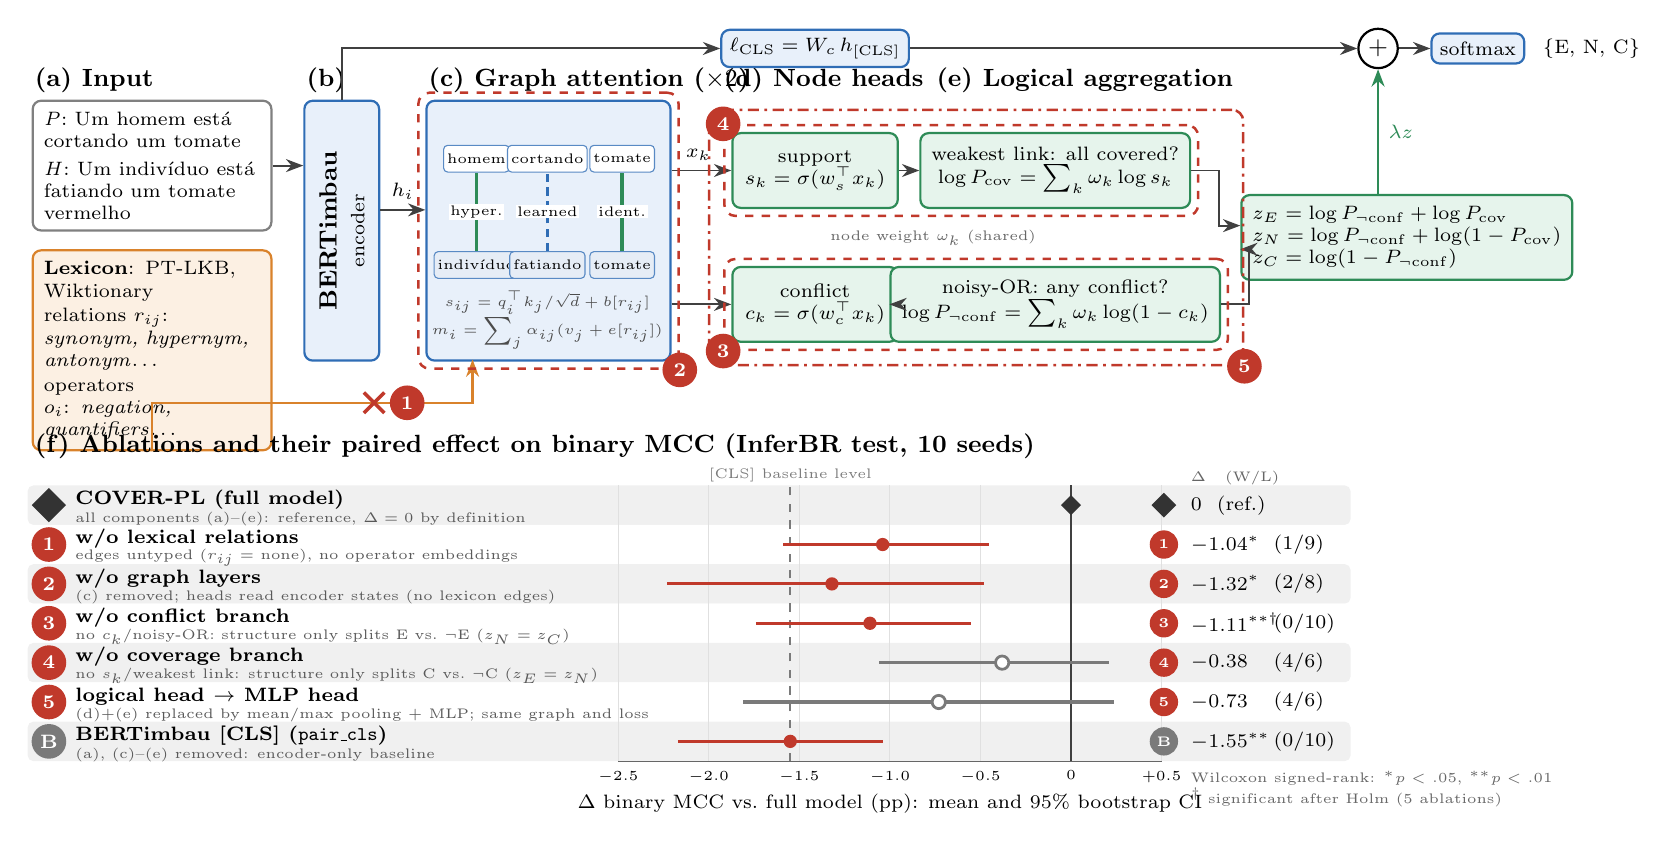
\begin{tikzpicture}[font=\small]

% =====================================================================
% Top: simplified architecture with ablation marks
% =====================================================================
% (a) input + lexicon
\node[title] at (0,7.15) {(a) Input};
\node[block, draw=black!50, fill=white, anchor=north west, text width=2.75cm, font=\scriptsize, align=left] (inp) at (0,7.1) {%
  \textit{P}: Um homem está cortando um tomate\\[2pt]
  \textit{H}: Um indivíduo está fatiando um tomate vermelho};
\node[sblock, anchor=north west, text width=2.75cm, font=\scriptsize, align=left] (lex) at (0,5.2) {%
  \textbf{Lexicon}: PT-LKB, Wiktionary\\[1pt]
  relations $r_{ij}$: \textit{synonym, hypernym, antonym}\ldots\\[1pt]
  operators $o_i$: \textit{negation, quantifiers}\ldots};

% (b) encoder
\node[nblock, minimum width=0.95cm, minimum height=3.3cm, anchor=north west] (enc) at (3.45,7.1) {};
\node[rotate=90, align=center] at (enc.center) {\textbf{BERTimbau}\\[-1pt]\scriptsize encoder};
\node[title] at (3.45,7.15) {(b)};
\draw[flow] (inp.east) -- (enc.west|-inp.east);

% (c) relational graph attention
\node[nblock, minimum width=3.1cm, minimum height=3.3cm, anchor=north west] (gnn) at (5.0,7.1) {};
\node[title] at (5.0,7.15) {(c) Graph attention ($\times2$)};
\node[gnode] (p1) at (5.65,6.35) {homem};
\node[gnode] (p2) at (6.55,6.35) {cortando};
\node[gnode] (p3) at (7.5,6.35) {tomate};
\node[hnode] (h1) at (5.65,5.0) {indivíduo};
\node[hnode] (h2) at (6.55,5.0) {fatiando};
\node[hnode] (h3) at (7.5,5.0) {tomate};
\draw[line width=1.3pt, draw=logic] (h1) -- node[lab] {hyper.} (p1);
\draw[line width=0.9pt, draw=neural, densely dashed] (h2) -- node[lab] {learned} (p2);
\draw[line width=1.6pt, draw=logic] (h3) -- node[lab] {ident.} (p3);
\node[font=\tiny, align=center, text=black!70] at (6.55,4.3) {$s_{ij}=q_i^{\top}k_j/\sqrt{d}+b[r_{ij}]$\\$m_i=\sum_j\alpha_{ij}(v_j+e[r_{ij}])$};
\draw[flow] (enc.east|-6.0,5.7) -- (gnn.west|-6.0,5.7) node[midway, above, font=\scriptsize] {$h_i$};

% lexicon -> graph, routed below the encoder (ablation 1 cuts it)
\draw[flow, draw=symb, line width=0.9pt] (lex.south) |- (5.6,3.25) -- (5.6,3.8);
\coordinate (cut1) at (4.35,3.25);

% (d) node heads and (e) aggregation: coverage lane (top) and conflict lane (bottom)
\def\covy{6.2} \def\cony{4.5}
\node[title] at (8.75,7.15) {(d) Node heads};
\node[title] at (11.45,7.15) {(e) Logical aggregation};
\node[lblock, minimum width=2.1cm, minimum height=0.95cm] (sk) at (9.95,\covy) {support\\ $s_k=\sigma(w_s^{\top}x_k)$};
\node[lblock, minimum width=2.1cm, minimum height=0.95cm] (ck) at (9.95,\cony) {conflict\\ $c_k=\sigma(w_c^{\top}x_k)$};
\node[lblock, minimum width=2.9cm, minimum height=0.95cm] (wl) at (13.0,\covy) {weakest link: all covered?\\ $\log P_{\mathrm{cov}}=\sum_k\omega_k\log s_k$};
\node[lblock, minimum width=2.9cm, minimum height=0.95cm] (nor) at (13.0,\cony) {noisy-OR: any conflict?\\ $\log P_{\neg\mathrm{conf}}=\sum_k\omega_k\log(1-c_k)$};
\node[font=\tiny, text=black!60] at (11.45,5.35) {node weight $\omega_k$ (shared)};
\draw[flow] (gnn.east|-sk) -- (sk.west) node[pos=0.45, above, font=\scriptsize] {$x_k$};
\draw[flow] (gnn.east|-ck) -- (ck.west);
\draw[flow] (sk) -- (wl);
\draw[flow] (ck) -- (nor);

% z and fusion
\node[lblock, font=\scriptsize, align=left, anchor=west] (z) at (15.35,5.35) {%
  $z_E=\log P_{\neg\mathrm{conf}}+\log P_{\mathrm{cov}}$\\
  $z_N=\log P_{\neg\mathrm{conf}}+\log(1-P_{\mathrm{cov}})$\\
  $z_C=\log(1-P_{\neg\mathrm{conf}})$};
\draw[flow] (wl.east) -- ++(0.35,0) |- ($(z.west)+(0,0.15)$);
\draw[flow] (nor.east) -- ++(0.35,0) |- ($(z.west)+(0,-0.15)$);

\def\band{7.75}
\node[nblock, font=\scriptsize, inner sep=3pt] (wc) at (9.95,\band) {$\ell_{\mathrm{CLS}}=W_c\,h_{[\mathrm{CLS}]}$};
\node[draw, circle, line width=0.8pt, inner sep=0pt, minimum size=5mm] (plus) at (17.1,\band) {$+$};
\node[nblock, font=\scriptsize, inner sep=3pt, right=0.4cm of plus] (soft) {softmax};
\draw[flow] (enc.north) |- (wc.west);
\draw[flow] (wc.east) -- (plus.west);
\draw[flow, draw=logic, line width=0.9pt] (z.north-|plus) -- (plus.south) node[midway, right, font=\scriptsize, text=logic] {$\lambda z$};
\draw[flow] (plus.east) -- (soft.west);
\node[font=\scriptsize, anchor=west] at ($(soft.east)+(0.1,0)$) {\{E, N, C\}};

% ---- ablation marks -----------------------------------------------------
\draw[abl, line width=1.3pt] ($(cut1)+(-0.13,-0.13)$) -- ($(cut1)+(0.13,0.13)$);
\draw[abl, line width=1.3pt] ($(cut1)+(-0.13,0.13)$) -- ($(cut1)+(0.13,-0.13)$);
\node[badge] at ($(cut1)+(0.42,0)$) {1};
\node[ablbox, fit=(gnn), inner sep=2.5pt] (a2) {};
\node[badge] at (a2.south east) {2};
\node[ablbox, dash pattern=on 4pt off 2pt on 1pt off 2pt, fit=(sk)(ck)(wl)(nor), inner sep=8pt] (a5) {};
\node[badge] at (a5.south east) {5};
\node[ablbox, fit=(ck)(nor), inner sep=2.5pt] (a3) {};
\node[badge] at (a3.south west) {3};
\node[ablbox, fit=(sk)(wl), inner sep=2.5pt] (a4) {};
\node[badge] at (a4.north west) {4};

% =====================================================================
% Bottom: what each ablation removes + paired effect on binary MCC
% =====================================================================
\begin{scope}[yshift=-1.2cm]
% zebra bands: one band per row, spanning labels, plot and numbers
\foreach \y/\c in {3.15/6, 2.65/0, 2.15/6, 1.65/0, 1.15/6, 0.65/0, 0.15/6}
  \fill[black!\c, rounded corners=2pt] (-0.05,\y-0.25) rectangle (16.75,\y+0.25);
\node[title] at (0,3.7) {(f) Ablations and their paired effect on binary MCC (InferBR test, 10 seeds)};

% #1 y, #2 badge, #3 name, #4 detail
\newcommand{\abrow}[4]{%
  \node[badge] at (0.22,#1) {#2};
  \node[anchor=west, font=\scriptsize\bfseries, inner sep=0] at (0.55,#1+0.07) {#3};
  \node[anchor=west, font=\tiny, text=black!65, inner sep=0] at (0.55,#1-0.17) {#4};
}
\node[diamond, fill=black!80, inner sep=0pt, minimum size=4.4mm] at (0.22,3.15) {};
\node[anchor=west, font=\scriptsize\bfseries, inner sep=0] at (0.55,3.22) {COVER-PL (full model)};
\node[anchor=west, font=\tiny, text=black!65, inner sep=0] at (0.55,2.98) {all components (a)--(e): reference, $\Delta=0$ by definition};
\abrow{2.65}{1}{w/o lexical relations}{edges untyped ($r_{ij}=$ none), no operator embeddings}
\abrow{2.15}{2}{w/o graph layers}{(c) removed; heads read encoder states (no lexicon edges)}
\abrow{1.65}{3}{w/o conflict branch}{no $c_k$/noisy-OR: structure only splits E vs.\ $\neg$E ($z_N=z_C$)}
\abrow{1.15}{4}{w/o coverage branch}{no $s_k$/weakest link: structure only splits C vs.\ $\neg$C ($z_E=z_N$)}
\abrow{0.65}{5}{logical head $\rightarrow$ MLP head}{(d)+(e) replaced by mean/max pooling + MLP; same graph and loss}
\node[badge, fill=mute] at (0.22,0.15) {B};
\node[anchor=west, font=\scriptsize\bfseries, inner sep=0] at (0.55,0.22) {BERTimbau [CLS] (\texttt{pair\_cls})};
\node[anchor=west, font=\tiny, text=black!65, inner sep=0] at (0.55,-0.02) {(a), (c)--(e) removed: encoder-only baseline};

% plot: Delta (pp) -> x = 13.2cm + 2.3cm * Delta
\begin{scope}[x=2.3cm, shift={(13.2cm,0)}]
  \foreach \t/\l in {-2.5/{$-2.5$},-2/{$-2.0$},-1.5/{$-1.5$},-1/{$-1.0$},-0.5/{$-0.5$},0/{$0$},0.5/{$+0.5$}} {
    \draw[black!12] (\t,-0.1) -- (\t,3.4);
    \node[font=\tiny, anchor=north] at (\t,-0.1) {\l};
  }
  \draw[black!60] (-2.5,-0.1) -- (0.5,-0.1);
  \draw[black!75, line width=0.8pt] (0,-0.1) -- (0,3.4);
  \draw[mute, dashed, line width=0.7pt] (-1.55,-0.1) -- (-1.55,3.4);
  \node[font=\tiny, anchor=south, text=mute, inner sep=1pt] at (-1.55,3.4) {[CLS] baseline level};
  \node[font=\scriptsize, anchor=north] at (-1.0,-0.4) {$\Delta$ binary MCC vs.\ full model (pp): mean and 95\% bootstrap CI};

  \newcommand{\sig}[4]{\draw[abl, line width=1.1pt] (#2,#1) -- (#3,#1); \fill[abl] (#4,#1) circle (2.4pt);}
  \newcommand{\nsg}[4]{\draw[mute, line width=1.1pt] (#2,#1) -- (#3,#1); \filldraw[fill=white, draw=mute, line width=1pt] (#4,#1) circle (2.4pt);}
  \node[diamond, fill=black!80, inner sep=0pt, minimum size=2.6mm] at (0,3.15) {};
  \sig{2.65}{-1.59}{-0.45}{-1.04}
  \sig{2.15}{-2.23}{-0.48}{-1.32}
  \sig{1.65}{-1.74}{-0.55}{-1.11}
  \nsg{1.15}{-1.06}{0.21}{-0.38}
  \nsg{0.65}{-1.81}{0.24}{-0.73}
  \sig{0.15}{-2.17}{-1.04}{-1.55}
\end{scope}

\node[anchor=west, font=\tiny, text=black!60] at (14.6,3.5) {$\Delta$\quad(W/L)};
\foreach \y/\b in {2.65/1, 2.15/2, 1.65/3, 1.15/4, 0.65/5}
  \node[badge, minimum size=3.6mm, font=\tiny\bfseries] at (14.38,\y) {\b};
\node[badge, minimum size=3.6mm, font=\tiny\bfseries, fill=mute] at (14.38,0.15) {B};
\node[diamond, fill=black!80, inner sep=0pt, minimum size=3.2mm] at (14.38,3.15) {};
\node[anchor=west, font=\scriptsize] at (14.6,3.15) {$0$\ \ (ref.)};
\foreach \y/\t in {2.65/{$-1.04^{*}$}, 2.15/{$-1.32^{*}$}, 1.65/{$-1.11^{**\dagger}$},
                  1.15/{$-0.38$}, 0.65/{$-0.73$}, 0.15/{$-1.55^{**}$}}
  \node[anchor=west, font=\scriptsize] at (14.6,\y) {\t};
\foreach \y/\t in {2.65/{1/9}, 2.15/{2/8}, 1.65/{0/10}, 1.15/{4/6}, 0.65/{4/6}, 0.15/{0/10}}
  \node[anchor=west, font=\scriptsize] at (15.65,\y) {(\t)};
\node[anchor=north west, font=\tiny, text=black!60, align=left] at (14.6,-0.1) {%
  Wilcoxon signed-rank: $^{*}p<.05$, $^{**}p<.01$\\ $^{\dagger}$ significant after Holm (5 ablations)};
\end{scope}

\end{tikzpicture}
\end{document}
